% Options for packages loaded elsewhere
\PassOptionsToPackage{unicode}{hyperref}
\PassOptionsToPackage{hyphens}{url}
%
\documentclass[
]{book}
\usepackage{lmodern}
\usepackage{amssymb,amsmath}
\usepackage{ifxetex,ifluatex}
\ifnum 0\ifxetex 1\fi\ifluatex 1\fi=0 % if pdftex
  \usepackage[T1]{fontenc}
  \usepackage[utf8]{inputenc}
  \usepackage{textcomp} % provide euro and other symbols
\else % if luatex or xetex
  \usepackage{unicode-math}
  \defaultfontfeatures{Scale=MatchLowercase}
  \defaultfontfeatures[\rmfamily]{Ligatures=TeX,Scale=1}
\fi
% Use upquote if available, for straight quotes in verbatim environments
\IfFileExists{upquote.sty}{\usepackage{upquote}}{}
\IfFileExists{microtype.sty}{% use microtype if available
  \usepackage[]{microtype}
  \UseMicrotypeSet[protrusion]{basicmath} % disable protrusion for tt fonts
}{}
\makeatletter
\@ifundefined{KOMAClassName}{% if non-KOMA class
  \IfFileExists{parskip.sty}{%
    \usepackage{parskip}
  }{% else
    \setlength{\parindent}{0pt}
    \setlength{\parskip}{6pt plus 2pt minus 1pt}}
}{% if KOMA class
  \KOMAoptions{parskip=half}}
\makeatother
\usepackage{xcolor}
\IfFileExists{xurl.sty}{\usepackage{xurl}}{} % add URL line breaks if available
\IfFileExists{bookmark.sty}{\usepackage{bookmark}}{\usepackage{hyperref}}
\hypersetup{
  pdftitle={Homework 1},
  pdfauthor={Chi-Yuan Fang},
  hidelinks,
  pdfcreator={LaTeX via pandoc}}
\urlstyle{same} % disable monospaced font for URLs
\usepackage{color}
\usepackage{fancyvrb}
\newcommand{\VerbBar}{|}
\newcommand{\VERB}{\Verb[commandchars=\\\{\}]}
\DefineVerbatimEnvironment{Highlighting}{Verbatim}{commandchars=\\\{\}}
% Add ',fontsize=\small' for more characters per line
\usepackage{framed}
\definecolor{shadecolor}{RGB}{248,248,248}
\newenvironment{Shaded}{\begin{snugshade}}{\end{snugshade}}
\newcommand{\AlertTok}[1]{\textcolor[rgb]{0.94,0.16,0.16}{#1}}
\newcommand{\AnnotationTok}[1]{\textcolor[rgb]{0.56,0.35,0.01}{\textbf{\textit{#1}}}}
\newcommand{\AttributeTok}[1]{\textcolor[rgb]{0.77,0.63,0.00}{#1}}
\newcommand{\BaseNTok}[1]{\textcolor[rgb]{0.00,0.00,0.81}{#1}}
\newcommand{\BuiltInTok}[1]{#1}
\newcommand{\CharTok}[1]{\textcolor[rgb]{0.31,0.60,0.02}{#1}}
\newcommand{\CommentTok}[1]{\textcolor[rgb]{0.56,0.35,0.01}{\textit{#1}}}
\newcommand{\CommentVarTok}[1]{\textcolor[rgb]{0.56,0.35,0.01}{\textbf{\textit{#1}}}}
\newcommand{\ConstantTok}[1]{\textcolor[rgb]{0.00,0.00,0.00}{#1}}
\newcommand{\ControlFlowTok}[1]{\textcolor[rgb]{0.13,0.29,0.53}{\textbf{#1}}}
\newcommand{\DataTypeTok}[1]{\textcolor[rgb]{0.13,0.29,0.53}{#1}}
\newcommand{\DecValTok}[1]{\textcolor[rgb]{0.00,0.00,0.81}{#1}}
\newcommand{\DocumentationTok}[1]{\textcolor[rgb]{0.56,0.35,0.01}{\textbf{\textit{#1}}}}
\newcommand{\ErrorTok}[1]{\textcolor[rgb]{0.64,0.00,0.00}{\textbf{#1}}}
\newcommand{\ExtensionTok}[1]{#1}
\newcommand{\FloatTok}[1]{\textcolor[rgb]{0.00,0.00,0.81}{#1}}
\newcommand{\FunctionTok}[1]{\textcolor[rgb]{0.00,0.00,0.00}{#1}}
\newcommand{\ImportTok}[1]{#1}
\newcommand{\InformationTok}[1]{\textcolor[rgb]{0.56,0.35,0.01}{\textbf{\textit{#1}}}}
\newcommand{\KeywordTok}[1]{\textcolor[rgb]{0.13,0.29,0.53}{\textbf{#1}}}
\newcommand{\NormalTok}[1]{#1}
\newcommand{\OperatorTok}[1]{\textcolor[rgb]{0.81,0.36,0.00}{\textbf{#1}}}
\newcommand{\OtherTok}[1]{\textcolor[rgb]{0.56,0.35,0.01}{#1}}
\newcommand{\PreprocessorTok}[1]{\textcolor[rgb]{0.56,0.35,0.01}{\textit{#1}}}
\newcommand{\RegionMarkerTok}[1]{#1}
\newcommand{\SpecialCharTok}[1]{\textcolor[rgb]{0.00,0.00,0.00}{#1}}
\newcommand{\SpecialStringTok}[1]{\textcolor[rgb]{0.31,0.60,0.02}{#1}}
\newcommand{\StringTok}[1]{\textcolor[rgb]{0.31,0.60,0.02}{#1}}
\newcommand{\VariableTok}[1]{\textcolor[rgb]{0.00,0.00,0.00}{#1}}
\newcommand{\VerbatimStringTok}[1]{\textcolor[rgb]{0.31,0.60,0.02}{#1}}
\newcommand{\WarningTok}[1]{\textcolor[rgb]{0.56,0.35,0.01}{\textbf{\textit{#1}}}}
\usepackage{longtable,booktabs}
% Correct order of tables after \paragraph or \subparagraph
\usepackage{etoolbox}
\makeatletter
\patchcmd\longtable{\par}{\if@noskipsec\mbox{}\fi\par}{}{}
\makeatother
% Allow footnotes in longtable head/foot
\IfFileExists{footnotehyper.sty}{\usepackage{footnotehyper}}{\usepackage{footnote}}
\makesavenoteenv{longtable}
\usepackage{graphicx,grffile}
\makeatletter
\def\maxwidth{\ifdim\Gin@nat@width>\linewidth\linewidth\else\Gin@nat@width\fi}
\def\maxheight{\ifdim\Gin@nat@height>\textheight\textheight\else\Gin@nat@height\fi}
\makeatother
% Scale images if necessary, so that they will not overflow the page
% margins by default, and it is still possible to overwrite the defaults
% using explicit options in \includegraphics[width, height, ...]{}
\setkeys{Gin}{width=\maxwidth,height=\maxheight,keepaspectratio}
% Set default figure placement to htbp
\makeatletter
\def\fps@figure{htbp}
\makeatother
\setlength{\emergencystretch}{3em} % prevent overfull lines
\providecommand{\tightlist}{%
  \setlength{\itemsep}{0pt}\setlength{\parskip}{0pt}}
\setcounter{secnumdepth}{5}
\usepackage{booktabs}
\usepackage{amsthm}
\makeatletter
\def\thm@space@setup{%
  \thm@preskip=8pt plus 2pt minus 4pt
  \thm@postskip=\thm@preskip
}
\makeatother
\usepackage[]{natbib}
\bibliographystyle{apalike}

\title{Homework 1}
\author{Chi-Yuan Fang}
\date{2021-02-25}

\begin{document}
\maketitle

{
\setcounter{tocdepth}{1}
\tableofcontents
}
\hypertarget{textbook-exercises}{%
\chapter{Textbook Exercises}\label{textbook-exercises}}

Do the following problem sets from Stock \& Watson (4th Edition).

2.6, 2.8, 2.14, 2.25, 3.2, 3.3, 3.4, 3.9, 3.13

\hypertarget{exercise-2.6}{%
\section{Exercise 2.6}\label{exercise-2.6}}

\begin{enumerate}
\def\labelenumi{\alph{enumi}.}
\item
  \begin{align}
        E(Y)
        & = 0\cdot 0.12 + 1\cdot 0.88 
          = 0.88
    \end{align}
\item
  \begin{align}
        Pr(Y = 0) 
        & = 1 - Pr(Y = 1) \\
        & = 1 - E(Y) \\
        & = 1 - 0.88
          = 0.12
    \end{align}
\item
  The conditional probabilities are
  \begin{align}
        Pr(Y = 0 \lvert X = 0)
        & = \frac{Pr(X=0,Y=0)}{Pr(X=0)} \\
        & = \frac{0.078}{0.751} 
          = \frac{78}{751} \\
        Pr(Y = 1 \lvert X = 0)
        & = \frac{Pr(X=0,Y=1)}{Pr(X=0)} \\
        & = \frac{0.673}{0.751} 
          = \frac{673}{751} \\
        Pr(Y = 0 \lvert X = 1)
        & = \frac{Pr(X=1,Y=0)}{Pr(X=1)} \\
        & = \frac{0.042}{0.249} 
          = \frac{14}{83} \\
        Pr(Y = 1 \lvert X = 1)
        & = \frac{Pr(X=1,Y=1)}{Pr(X=1)} \\
        & = \frac{0.207}{0.249} 
          = \frac{69}{83}.   
    \end{align}
  Then, the conditional expectations are
  \begin{align}
        E(Y \lvert X = 1)
        & = 0\cdot \frac{14}{83} + 1\cdot \frac{69}{83}
          = \frac{69}{83} 
          \approx 0.8313 \\
        E(Y \lvert X = 0)
        & = 0\cdot \frac{78}{751} + 1\cdot \frac{673}{751}
          = \frac{673}{751} 
          \approx 0.8961.
    \end{align}
\item
  Unemployment rate for college graduates is
  \begin{align}
        Pr(Y = 0 \lvert X = 1)
        & = 1 - E(Y \lvert X = 1) \\
        & = 1 - \frac{69}{83} \\
        & = \frac{14}{83}
          \approx 0.1687,
    \end{align}
  and unemployment rate for non-college graduates is
  \begin{align}
        Pr(Y = 0 \lvert X = 0)
        & = 1 - E(Y \lvert X = 0) \\
        & = 1 - \frac{673}{751}  \\
        & = \frac{78}{751}
          \approx 0.1039.
    \end{align}
\item
  Given a randomly selected member of unemployed population, the probability that the worker is a college graduate is
  \begin{align}
        Pr(X = 1 \lvert Y = 0)
        & = \frac{Pr(X = 1, Y = 0)}{Pr(Y = 0)} \\
        & = \frac{0.042}{0.12} 
          = 0.35,
    \end{align}
  and the probability that the worker is a non-college graduate is
  \begin{align}
        Pr(X = 0 \lvert Y = 0)
        & = \frac{Pr(X = 0, Y = 0)}{Pr(Y = 0)} \\
        & = \frac{0.078}{0.12} 
          = 0.65.
    \end{align}
\item
  Because
  \begin{align}
        Pr(X = 0\lvert Y = 0)
        & = \frac{78}{751} \\
        & \neq Pr(X = 0) = 0.12,
    \end{align}
  educational achievement and employment status are not independent.
\end{enumerate}

\hypertarget{exercise-2.8}{%
\section{Exercise 2.8}\label{exercise-2.8}}

We know
\begin{align}
    E(Y) = 4 \quad \mbox{and} \quad Var(Y) = \frac{1}{9}.
\end{align}
Then,
\begin{align}
    E(Z) 
    & = E\left[ 3(Y - 4) \right] \\
    & = 3E(Y - 4) \\
    & = 3E(Y) - 12 \\
    & = 3\cdot 4 - 12 = 0
\end{align}
and
\begin{align}
    Var(Z)
    & = Var\left[ 3(Y - 4) \right] \\
    & = 3^2 \cdot Var(Y - 4) \\
    & = 9\cdot Var(Y) \\
    & = 9\cdot \frac{1}{9}
      = 1.
\end{align}

\hypertarget{exercise-2.14}{%
\section{Exercise 2.14}\label{exercise-2.14}}

By CLT, we have
\begin{align}
    \overline{Y}
    \sim
    N\left(\mu_Y, \frac{\sigma_Y^2}{n}\right)
    \stackrel{d}{=}
    N\left(50, \frac{21}{n} \right).
\end{align}

\begin{enumerate}
\def\labelenumi{\alph{enumi}.}
\item
  \begin{align}
        Pr\left( \overline{Y}\leq 51 \right)
        & = Pr\left( \frac{\overline{Y} - 50}{\sqrt{21/50}} \leq \frac{51 - 50}{\sqrt{21/50}}\right) 
          \approx 0.9386
    \end{align}
\item
  \begin{align}
        Pr\left( \overline{Y} > 49 \right)
        & = Pr\left( \frac{\overline{Y} - 50}{\sqrt{21/150}} > \frac{49 - 50}{\sqrt{21/150}}\right) 
          \approx 0.9962
    \end{align}
\item
  \begin{align}
        Pr\left( 50.5 \leq \overline{Y} < 51 \right)
        & = Pr\left( \frac{50.5 - 50}{\sqrt{21/45}} \leq \overline{Y} \leq \frac{51 - 50}{\sqrt{21/45}}\right) 
          \approx 0.1605
    \end{align}
\end{enumerate}

\hypertarget{exercise-2.25}{%
\section{Exercise 2.25}\label{exercise-2.25}}

\begin{enumerate}
\def\labelenumi{\alph{enumi}.}
\item
  \begin{align}
        \sum_{i=1}^{n}ax_i 
        & = ax_1 + ax_2 + \ldots + ax_n \\
        & = a(x_1 + x_2 + \ldots + x_n) \\
        & = a\sum_{i=1}^{n}x_i
    \end{align}
\item
  \begin{align}
        \sum_{i=1}^{n}(x_i + y_i) 
        & = (x_1 + y_1) + (x_2 + y_2) + \ldots + (x_n + y_n) \\
        & = (x_1 + x_2 + \ldots + x_n) + (y_1 + y_2 + \ldots + y_n) \\
        & = \sum_{i=1}^{n} x_i + \sum_{i=1}^{n} y_i
    \end{align}
\item
  \begin{align}
        \sum_{i=1}^{n} a
        & = \underbrace{a + a + \ldots + a}_{n\mbox{ times}} \\
        & = n\times a
    \end{align}
\item
  \begin{align}
        \sum_{i=1}^{n} (a + bx_i + cy_i)^2 
        & = \sum_{i=1}^{n} \left( a^2 + b^2x_i^2 + c^2y_i^2 + 2abx_i + 2acy_i + 2bcx_iy_i \right) \\
        & = na^2 + b^2\sum_{i=1}^{n}x_i^2 + c^2\sum_{i=1}^{n}y_i^2 + 2ab\sum_{i=1}^{n}x_i + 2ac\sum_{i=1}^{n}y_i + 2bc\sum_{i=1}^{n}x_iy_i
    \end{align}
\end{enumerate}

\hypertarget{exercise-3.2}{%
\section{Exercise 3.2}\label{exercise-3.2}}

\begin{enumerate}
\def\labelenumi{\alph{enumi}.}
\item
  \begin{align}
       \widehat{p}
       & = \frac{1}{n} \sum_{i=1}^{n}Y_i
         = \overline{Y}
   \end{align}
\item
  \begin{align}
        E\left( \widehat{p} \right)
        & = E\left( \overline{Y} \right) \\
        & = E\left( \frac{1}{n}\sum_{i=1}^{n} Y_i \right) \\
        & = \frac{1}{n} E\left( \sum_{i=1}^{n} Y_i \right) \\
        & = \frac{1}{n} \sum_{i=1}^{n} E(Y_i) \\
        & = \frac{1}{n}\cdot np
          = p
    \end{align}
\item
  \begin{align}
        Var\left( \widehat{p} \right)
        & = Var\left( \overline{Y} \right) \\
        & = Var\left( \frac{1}{n}\sum_{i=1}^{n}Y_i \right) \\
        & = \frac{1}{n^2} Var\left( \sum_{i=1}^{n}Y_i \right) \\
        & = \frac{1}{n^2} \left[ nVar(Y_i) + 2\sum_{i\neq j} \underbrace{Cov (Y_i, Y_j)}_{=0} \right] \\
        & = \frac{1}{n^2} \cdot np(1-p) 
          = \frac{p(1-p)}{n}
    \end{align}
\end{enumerate}

\hypertarget{exercise-3.3}{%
\section{Exercise 3.3}\label{exercise-3.3}}

\begin{enumerate}
\def\labelenumi{\alph{enumi}.}
\item
  \begin{align}
       \widehat{p}
       & = \frac{270}{500} 
         = 0.54
   \end{align}
\item
  The estimated variance of \(\widehat{p}\) is
  \begin{align}
        Var\left( \widehat{p} \right)
        & = \frac{\widehat{p} \left( 1 -\widehat{p} \right)}{n} \\
        & = \frac{0.54(1-0.54)}{500}  
          = 0.0004968,
    \end{align}
  and the standard error is
  \begin{align}
        SE\left( \widehat{p} \right)
        & = \sqrt{Var\left( \widehat{p} \right)} \\
        & \approx 0.0223.
    \end{align}
\item
  The \(t\)-statistic is
  \begin{align}
        t^* 
        & = \frac{\widehat{p} - p_0}{SE\left( \widehat{p} \right)} \\
        & = \frac{0.54 - 0.5}{0.0223} \\
        & = \frac{400}{223} 
          \approx 1.7937.
    \end{align}
  Then,
  \begin{align}
        p-value
        & = 2\Phi \left( -\lvert{t^*}\lvert \right) \\
        & = 2\Phi \left( -\frac{400}{223} \right) 
          \approx 0.0729.
    \end{align}
\item
  The \(t\)-statistic is
  \begin{align}
        t^* 
        & = \frac{\widehat{p} - p_0}{SE\left( \widehat{p} \right)} \\
        & = \frac{0.54 - 0.5}{0.0223} \\
        & = \frac{400}{223} 
          \approx 1.7937.
    \end{align}
  Then,
  \begin{align}
        p-value
        & = 1 - \Phi \left( \lvert{t^*}\lvert \right) \\
        & = 1 - \Phi \left( \frac{400}{223} \right) 
          \approx 0.0364.
    \end{align}
\item
  Part (c) is a two-sided test and the p-value is the area in the tails of the standard normal distribution outside the \(\pm\) (calculated \(t\)-statistic). Part (d) is a one-sided test
  and the p-value is the area under the standard normal distribution to the right of the calculated \(t\)-statistic.
\item
  For the test \(H_0: p = 0.5\) vs.~\(H_1: p > 0.5\) and \(\alpha = 0.05\), we reject \(H_0\) because \(p\)-value is less than the significance level. There is statistically significant evidence that the democratic candidate was ahead of the republican candidate at the time of conducting the poll.
\end{enumerate}

\hypertarget{exercise-3.4}{%
\section{Exercise 3.4}\label{exercise-3.4}}

\begin{enumerate}
\def\labelenumi{\alph{enumi}.}
\item
  \begin{align}
        \overline{p} \pm Z_{0.025}SE\left( \overline{p} \right) 
        & = 0.54 \pm 1.96\cdot 0.0223
          \approx [0.4963,0.5837]
    \end{align}
\item
  \begin{align}
        \overline{p} \pm Z_{0.005}SE\left( \overline{p} \right) 
        & = 0.54 \pm 2.576\cdot 0.0223
          \approx [0.4826,0.5974]
    \end{align}
\item
  Mechanically, the interval in part (b) is wider because of a larger critical value. Substantively, a 99\% confidence interval is wider than a 95\% confidence level because a 99\% confidence interval must contain the true value of \(p\) in 99\% of all possible samples, while a 95\% confidence interval must contain the true value of \(p\) in only 95\% of all possible samples.
\item
  Because \(0.5\in C.I.\), we do not reject \(H_0\) at \(5\%\) significance level.
\end{enumerate}

\hypertarget{exercise-3.9}{%
\section{Exercise 3.9}\label{exercise-3.9}}

\begin{enumerate}
\def\labelenumi{\alph{enumi}.}
\item
  We know
  \begin{align}
        E(Y) & = 1000 \\
        \sigma_Y & = 100 \\
        n & = 50
    \end{align}
  and
  \begin{align}
        E\left(\overline{Y} \right) & = 1000 \\
        \sigma_{\overline{Y}} & = \frac{100}{\sqrt{50}}
                                = 10\sqrt{2}.
    \end{align}
  Then,
  \begin{align}
        \mbox{size} 
        & = \Pr\left( \overline{Y} > 1100 \lvert \mu = 1000 \right) \\
        & = \Pr\left( \frac{\overline{Y} - 1000}{10\sqrt{2}} > \frac{1100 - 1000}{10\sqrt{2}} \right) 
          \approx 0.
    \end{align}
\item
  The probability of type 2 error is
  \begin{align}
        \beta
        & = \Pr\left( \overline{Y} \lvert \mu = 1150 \right) \\
        & = \Pr\left( \frac{\overline{Y} - 1150}{10\sqrt{2}} \leq \frac{1100 - 1150}{10\sqrt{2}} \right) 
          \approx 0.0002.
    \end{align}
  Then, the power of the manager's testing is
  \begin{align}
        1-\beta 
        & \approx 0.9998.
    \end{align}
\item
  For a test with size 1\%, the rejection region for \(H_0\) contains those values of the \(t\)-statistic exceeding \(Z_{0.01}\). That is,
  \begin{align}
        t^* 
        & = \frac{\overline{Y} - 1000}{10\sqrt{2}}
          > Z_{0.01} = 2.326.
    \end{align}

  Then,
  \begin{align}
        \overline{Y}
        & > 1000 + 10\sqrt{2}\cdot 2.326
          \approx 1032.8946.
    \end{align}

  Thus, the manager should believe the inventor's claim if the sample mean life of the new product is greater than 1032.8946 hours if she wants the size of the test to be 1\%.
\end{enumerate}

\hypertarget{exercise-3.13}{%
\section{Exercise 3.13}\label{exercise-3.13}}

\begin{enumerate}
\def\labelenumi{\alph{enumi}.}
\item
  \begin{align}
        \overline{Y} \pm Z_{0.05}\cdot \frac{s_Y}{\sqrt{n}}
        & = 712.1 \pm 1.645 \cdot \frac{23.2}{\sqrt{400}}
          = [710.1918, 714.0082]
    \end{align}
\item
\end{enumerate}

\begin{itemize}
\item
  \textbf{Prepare}:
  \(H_0: \mu_1 - \mu_2 = 0\) vs.~\(H_1: \mu_1 - \mu_2 \neq 0\), where \(\mu_1\) is average salary with small class, \(\mu_2\) is average salary with large class. Let the significance level be \(0.05\).
\item
  \textbf{Calculate}:
  \begin{align}
      t^*
      & = \frac{\left( \overline{Y}_1 - \overline{Y}_2 \right) - 0}{\sqrt{\frac{s_1^2}{n_1} + \frac{s_2^2}{n_2}}} \\
      & = \frac{721.8 - 710.9}{\sqrt{\frac{24.4^2}{150}+ \frac{20.6}{250}}} 
        \approx 4.5790
  \end{align}
\item
  \textbf{Conclude}:
  Because
  \begin{align}
      t^* > Z_{0.025} = 1.96,
  \end{align}
  we reject \(H_0\). There is statistically significant evidence that districts with smaller classes have higher average test scores.
\end{itemize}

\hypertarget{computer-exercises}{%
\chapter{Computer exercises}\label{computer-exercises}}

Do the following problem set from Stock \& Watson (4th Edition).

E3.2

\hypertarget{e3.2}{%
\section{E3.2}\label{e3.2}}

\begin{quote}
A consumer is given the chance to buy a baseball card for \$1, but he declines
the trade. If the consumer is now given the baseball card, will he be willing to sell it for \$1? Standard consumer theory suggests yes, but behavioral economists have found that ``ownership'' tends to increase the value of goods to
consumers. That is, the consumer may hold out for some amount more than
\$1 (for example, \$1.20) when selling the card, even though he was willing
to pay only some amount less than \$1 (for example, \$0.88) when buying it.
Behavioral economists call this phenomenon the ``endowment effect.'' John
List investigated the endowment effect in a randomized experiment involving
sports memorabilia traders at a sports-card show. Traders were randomly
given one of two sports collectibles, say good A or good B, that had approximately equal market value. Those receiving good A were then given the
option of trading good A for good B with the experimenter; those receiving
good B were given the option of trading good B for good A with the
experimenter. Data from the experiment and a detailed description can be
found on the text website, \url{http://www.pearsonglobaleditions.com}, in the files \textbf{Sportscards and Sportscards\_Description}.
\end{quote}

\begin{quote}
\begin{enumerate}
\def\labelenumi{\alph{enumi}.}
\item
  \begin{enumerate}
  \def\labelenumii{\roman{enumii}.}
  \tightlist
  \item
    Suppose that, absent any endowment effect, all the subjects prefer good A to good B. What fraction of the experiment's subjects would you expect to trade the good that they were given for the other good? (Hint:
    Because of random assignment of the two treatments, approximately 50\% of the subjects received good A, and 50\% received good B.)
  \item
    Suppose that, absent any endowment effect, 50\% of the subjects prefer good A to good B, and the other 50\% prefer good B to good A. What fraction of the subjects would you expect to trade the good they were given for the other good?
  \item
    Suppose that, absent any endowment effect, \(X\%\) of the subjects prefer good A to good B, and the other \((100 - X)\%\) prefer good B to good A. Show that you would expect 50\% of the subjects to trade the good they were given for the other good.
  \end{enumerate}
\end{enumerate}
\end{quote}

\textbf{Solution}

\begin{enumerate}
\def\labelenumi{\roman{enumi}.}
\item
  A person will trade if he/she received good A but prefers good B or he/she received good B and prefers good A. 50\% received good A, of these \(100\%\) prefer good B; 50\% receive good B, of these \(0\%\) prefer good A. Thus, the expected fraction traded is
  \begin{align}
  0.5 \times 1 + 0.5\times 0 = 0.5.
  \end{align}
\item
  A person will trade if he/she received good A but prefers good B or he/she received good B and prefers good A. 50\% received good A, of these \(50\%\) prefer good B; 50\% receive good B, of these \(50\%\) prefer good A. Thus, the expected fraction traded is
  \begin{align}
  0.5 \times 0.5 + 0.5\times 0.5 = 0.5.
  \end{align}
\item
  A person will trade if he/she received good A but prefers good B or he/she received good B and prefers good A. 50\% received good A, of these \((100-X)\%\) prefer good B; 50\% receive good B, of these \(X\%\) prefer good A. Thus, the expected fraction traded is
  \begin{align}
  0.5 \times (1-x) + 0.5x = 0.5
  \end{align}
  where \(x = \frac{X}{100}\).
\end{enumerate}

\begin{quote}
\begin{enumerate}
\def\labelenumi{\alph{enumi}.}
\setcounter{enumi}{1}
\tightlist
\item
  Using the sports-card data, what fraction of the subjects traded the good they were given? Is the fraction significantly different from 50\%? Is there evidence of an endowment effect? (Hint: Review Exercises 3.2 and 3.3.)
\end{enumerate}
\end{quote}

\textbf{Solution}

\begin{itemize}
\tightlist
\item
  \textbf{Prepare}
\end{itemize}

\(H_0: p= 0.5\) (no endowment effect) v.s. \(H_A: p \neq 0.5\) (endowment effect), where \(p\) is the fraction of trades.

Let the significance level be \(0.05\).

\begin{itemize}
\tightlist
\item
  \textbf{Calculate}
\end{itemize}

\begin{Shaded}
\begin{Highlighting}[]
\CommentTok{# import data }
\KeywordTok{library}\NormalTok{(readxl)}
\NormalTok{sportscards <-}\StringTok{ }\KeywordTok{read_xlsx}\NormalTok{(}\StringTok{"sportscards/Sportscards.xlsx"}\NormalTok{)}

\CommentTok{# the fraction of trades}
\NormalTok{fract_trade <-}\StringTok{ }\KeywordTok{mean}\NormalTok{(sportscards}\OperatorTok{$}\NormalTok{trade)}
\NormalTok{fract_trade}
\end{Highlighting}
\end{Shaded}

\begin{verbatim}
## [1] 0.3378378
\end{verbatim}

\begin{Shaded}
\begin{Highlighting}[]
\CommentTok{# standard error of the fraction of trades}
\NormalTok{se_fract_trade <-}\StringTok{ }\KeywordTok{sd}\NormalTok{(sportscards}\OperatorTok{$}\NormalTok{trade)}\OperatorTok{/}\KeywordTok{sqrt}\NormalTok{(}\KeywordTok{length}\NormalTok{(sportscards}\OperatorTok{$}\NormalTok{trade))}
\NormalTok{se_fract_trade}
\end{Highlighting}
\end{Shaded}

\begin{verbatim}
## [1] 0.03901015
\end{verbatim}

\begin{Shaded}
\begin{Highlighting}[]
\CommentTok{# test}
\KeywordTok{t.test}\NormalTok{(sportscards}\OperatorTok{$}\NormalTok{trade, }
       \DataTypeTok{alternative =} \KeywordTok{c}\NormalTok{(}\StringTok{"two.sided"}\NormalTok{),}
       \DataTypeTok{mu =} \FloatTok{0.5}\NormalTok{, }\CommentTok{# H0}
       \DataTypeTok{conf.level =} \FloatTok{0.95}\NormalTok{) }\CommentTok{# alpha = 0.05}
\end{Highlighting}
\end{Shaded}

\begin{verbatim}
## 
##  One Sample t-test
## 
## data:  sportscards$trade
## t = -4.1569, df = 147, p-value = 5.456e-05
## alternative hypothesis: true mean is not equal to 0.5
## 95 percent confidence interval:
##  0.2607447 0.4149310
## sample estimates:
## mean of x 
## 0.3378378
\end{verbatim}

\begin{itemize}
\tightlist
\item
  \textbf{Conclude}
\end{itemize}

The fraction of trades in the sample was 0.3378, with a standard error of 0.0390.

Because \(p-value < 0.05\), we reject \(H_0\). There is statistically significant evidence of an endowment effect.

\begin{quote}
\begin{enumerate}
\def\labelenumi{\alph{enumi}.}
\setcounter{enumi}{2}
\tightlist
\item
  Some have argued that the endowment effect may be present but that it is likely to disappear as traders gain more trading experience. Half of the experimental subjects were dealers, and the other half were nondealers. Dealers have more experience than nondealers. Repeat (b) for dealers and nondealers. Is there a significant difference in their behavior? Is the evidence consistent with the hypothesis that the endowment effect disappears as traders gain more experience? (Hint: Review Exercise 3.15.)
\end{enumerate}
\end{quote}

\textbf{Solution}

\begin{enumerate}
\def\labelenumi{\roman{enumi}.}
\tightlist
\item
  Dealers:
\end{enumerate}

\begin{itemize}
\tightlist
\item
  \textbf{Prepare}
\end{itemize}

\(H_0: p_1 = 0.5\) (no endowment effect) v.s. \(H_A: p_1 \neq 0.5\) (endowment effect), where \(p_1\) is the fraction of trades for dealers.

Let the significance level be \(0.05\).

\begin{itemize}
\tightlist
\item
  \textbf{Calculate}
\end{itemize}

\begin{Shaded}
\begin{Highlighting}[]
\CommentTok{# dealer}
\NormalTok{sportscards_dealer <-}\StringTok{ }\NormalTok{sportscards[sportscards}\OperatorTok{$}\NormalTok{dealer }\OperatorTok{==}\StringTok{ }\DecValTok{1}\NormalTok{,]}

\CommentTok{# the fraction of trades for dealers}
\NormalTok{fract_trade_dealer <-}\StringTok{ }\KeywordTok{mean}\NormalTok{(sportscards_dealer}\OperatorTok{$}\NormalTok{trade)}
\NormalTok{fract_trade_dealer}
\end{Highlighting}
\end{Shaded}

\begin{verbatim}
## [1] 0.4459459
\end{verbatim}

\begin{Shaded}
\begin{Highlighting}[]
\CommentTok{# standard error of the fraction of trades for dealers}
\NormalTok{se_fract_trade_dealer <-}\StringTok{ }\KeywordTok{sd}\NormalTok{(sportscards_dealer}\OperatorTok{$}\NormalTok{trade)}\OperatorTok{/}\KeywordTok{sqrt}\NormalTok{(}\KeywordTok{length}\NormalTok{(sportscards_dealer}\OperatorTok{$}\NormalTok{trade))}
\NormalTok{se_fract_trade_dealer}
\end{Highlighting}
\end{Shaded}

\begin{verbatim}
## [1] 0.05817759
\end{verbatim}

\begin{Shaded}
\begin{Highlighting}[]
\CommentTok{# test}
\KeywordTok{t.test}\NormalTok{(sportscards_dealer}\OperatorTok{$}\NormalTok{trade, }
       \DataTypeTok{alternative =} \KeywordTok{c}\NormalTok{(}\StringTok{"two.sided"}\NormalTok{),}
       \DataTypeTok{mu =} \FloatTok{0.5}\NormalTok{, }\CommentTok{# H0}
       \DataTypeTok{conf.level =} \FloatTok{0.95}\NormalTok{) }\CommentTok{# alpha = 0.05}
\end{Highlighting}
\end{Shaded}

\begin{verbatim}
## 
##  One Sample t-test
## 
## data:  sportscards_dealer$trade
## t = -0.92912, df = 73, p-value = 0.3559
## alternative hypothesis: true mean is not equal to 0.5
## 95 percent confidence interval:
##  0.3299982 0.5618937
## sample estimates:
## mean of x 
## 0.4459459
\end{verbatim}

\begin{itemize}
\tightlist
\item
  \textbf{Conclude}
\end{itemize}

The fraction of trades for dealers in the sample was 0.4459, with a standard error of 0.05818.

Because \(p-value > 0.05\), we don't reject \(H_0\). There is no evidence of an endowment effect.

\begin{enumerate}
\def\labelenumi{\roman{enumi}.}
\setcounter{enumi}{1}
\tightlist
\item
  Nondealers:
\end{enumerate}

\begin{itemize}
\tightlist
\item
  \textbf{Prepare}
\end{itemize}

\(H_0: p_2 = 0.5\) (no endowment effect) v.s. \(H_A: p_2 \neq 0.5\) (endowment effect), where \(p_2\) is the fraction of trades for nondealers.

Let the significance level be \(0.05\).

\begin{itemize}
\tightlist
\item
  \textbf{Calculate}
\end{itemize}

\begin{Shaded}
\begin{Highlighting}[]
\CommentTok{# nondealer }
\NormalTok{sportscards_nondealer <-}\StringTok{ }\NormalTok{sportscards[sportscards}\OperatorTok{$}\NormalTok{dealer }\OperatorTok{==}\StringTok{ }\DecValTok{0}\NormalTok{,]}

\CommentTok{# the fraction of trades for nondealers}
\NormalTok{fract_trade_nondealer <-}\StringTok{ }\KeywordTok{mean}\NormalTok{(sportscards_nondealer}\OperatorTok{$}\NormalTok{trade)}
\NormalTok{fract_trade_nondealer}
\end{Highlighting}
\end{Shaded}

\begin{verbatim}
## [1] 0.2297297
\end{verbatim}

\begin{Shaded}
\begin{Highlighting}[]
\CommentTok{# standard error of the fraction of trades for nondealers}
\NormalTok{se_fract_trade_nondealer <-}\StringTok{ }\KeywordTok{sd}\NormalTok{(sportscards_nondealer}\OperatorTok{$}\NormalTok{trade)}\OperatorTok{/}\KeywordTok{sqrt}\NormalTok{(}\KeywordTok{length}\NormalTok{(sportscards_nondealer}\OperatorTok{$}\NormalTok{trade))}
\NormalTok{se_fract_trade_nondealer}
\end{Highlighting}
\end{Shaded}

\begin{verbatim}
## [1] 0.04923441
\end{verbatim}

\begin{Shaded}
\begin{Highlighting}[]
\CommentTok{# test}
\KeywordTok{t.test}\NormalTok{(sportscards_nondealer}\OperatorTok{$}\NormalTok{trade, }
       \DataTypeTok{alternative =} \KeywordTok{c}\NormalTok{(}\StringTok{"two.sided"}\NormalTok{),}
       \DataTypeTok{mu =} \FloatTok{0.5}\NormalTok{, }\CommentTok{# H0}
       \DataTypeTok{conf.level =} \FloatTok{0.95}\NormalTok{) }\CommentTok{# alpha = 0.05}
\end{Highlighting}
\end{Shaded}

\begin{verbatim}
## 
##  One Sample t-test
## 
## data:  sportscards_nondealer$trade
## t = -5.4895, df = 73, p-value = 5.559e-07
## alternative hypothesis: true mean is not equal to 0.5
## 95 percent confidence interval:
##  0.1316057 0.3278538
## sample estimates:
## mean of x 
## 0.2297297
\end{verbatim}

\begin{itemize}
\tightlist
\item
  \textbf{Conclude}
\end{itemize}

The fraction of trades for nondealers in the sample was 0.2297, with a standard error of 0.0492.

Because \(p-value < 0.05\), we reject \(H_0\). There is statistically significant evidence of an endowment effect.

\begin{enumerate}
\def\labelenumi{\roman{enumi}.}
\setcounter{enumi}{2}
\tightlist
\item
  Difference between dealers and nondealers:
\end{enumerate}

\begin{itemize}
\tightlist
\item
  \textbf{Prepare}
\end{itemize}

\(H_0: p_1 - p_2 = 0\) v.s. \(H_A: p_1 - p_2 \neq 0\), where \(p_1\) is the fraction of trades for dealers, and \(p_2\) is the fraction of trades for nondealers.

Let the significance level be \(0.05\).

\begin{itemize}
\tightlist
\item
  \textbf{Calculate}
\end{itemize}

\begin{Shaded}
\begin{Highlighting}[]
\CommentTok{# difference}
\NormalTok{trade_diff <-}\StringTok{ }\NormalTok{sportscards_dealer}\OperatorTok{$}\NormalTok{trade }\OperatorTok{-}\StringTok{ }\NormalTok{sportscards_nondealer}\OperatorTok{$}\NormalTok{trade}

\CommentTok{# the fraction of trades for nondealers}
\NormalTok{fract_trade_diff <-}\StringTok{ }\KeywordTok{mean}\NormalTok{(trade_diff)}
\NormalTok{fract_trade_diff}
\end{Highlighting}
\end{Shaded}

\begin{verbatim}
## [1] 0.2162162
\end{verbatim}

\begin{Shaded}
\begin{Highlighting}[]
\CommentTok{# standard error of the fraction of trades for nondealers}
\NormalTok{se_fract_trade_diff <-}\StringTok{ }\KeywordTok{sd}\NormalTok{(trade_diff)}\OperatorTok{/}\KeywordTok{sqrt}\NormalTok{(}\KeywordTok{length}\NormalTok{(trade_diff))}
\NormalTok{se_fract_trade_diff}
\end{Highlighting}
\end{Shaded}

\begin{verbatim}
## [1] 0.07268651
\end{verbatim}

\begin{Shaded}
\begin{Highlighting}[]
\KeywordTok{t.test}\NormalTok{(trade_diff, }
       \DataTypeTok{alternative =} \KeywordTok{c}\NormalTok{(}\StringTok{"two.sided"}\NormalTok{),}
       \DataTypeTok{mu =} \FloatTok{0.5}\NormalTok{, }\CommentTok{# H0}
       \DataTypeTok{conf.level =} \FloatTok{0.95}\NormalTok{) }\CommentTok{# alpha = 0.05}
\end{Highlighting}
\end{Shaded}

\begin{verbatim}
## 
##  One Sample t-test
## 
## data:  trade_diff
## t = -3.9042, df = 73, p-value = 0.0002088
## alternative hypothesis: true mean is not equal to 0.5
## 95 percent confidence interval:
##  0.07135221 0.36108022
## sample estimates:
## mean of x 
## 0.2162162
\end{verbatim}

\begin{itemize}
\tightlist
\item
  \textbf{Conclude}
\end{itemize}

Because \(p-value < 0.05\), we reject \(H_0\). There is statistically significant difference in the behavior of Traders and non-Traders.

\hypertarget{introduction}{%
\chapter{Introduction}\label{introduction}}

\hypertarget{ta-information}{%
\section{TA Information}\label{ta-information}}

TA: Chi-Yuan Fang

TA sessions: Tuesday 1:20 -- 3:10 PM (SS 501)

Email: \href{mailto:r09323017@ntu.edu.tw}{\nolinkurl{r09323017@ntu.edu.tw}}

Office hours: Tuesday 3:20 - 4:10 PM or by appointments (SS 643)

Class group on Facebook: Statistics with Recitation (Fall 2020) \url{https://www.facebook.com/groups/452292659024369/}

Because screens are not clear in SS 501, I would provide live screen in the group.

\hypertarget{ta-sessions-schedule}{%
\section{TA Sessions Schedule}\label{ta-sessions-schedule}}

\begin{longtable}[]{@{}lllll@{}}
\toprule
\begin{minipage}[b]{0.08\columnwidth}\raggedright
Week\strut
\end{minipage} & \begin{minipage}[b]{0.17\columnwidth}\raggedright
TA Sessions\strut
\end{minipage} & \begin{minipage}[b]{0.08\columnwidth}\raggedright
Quiz\strut
\end{minipage} & \begin{minipage}[b]{0.32\columnwidth}\raggedright
Content\strut
\end{minipage} & \begin{minipage}[b]{0.22\columnwidth}\raggedright
Remind\strut
\end{minipage}\tabularnewline
\midrule
\endhead
\begin{minipage}[t]{0.08\columnwidth}\raggedright
1\strut
\end{minipage} & \begin{minipage}[t]{0.17\columnwidth}\raggedright
09/15: No class\strut
\end{minipage} & \begin{minipage}[t]{0.08\columnwidth}\raggedright
\strut
\end{minipage} & \begin{minipage}[t]{0.32\columnwidth}\raggedright
\strut
\end{minipage} & \begin{minipage}[t]{0.22\columnwidth}\raggedright
\strut
\end{minipage}\tabularnewline
\begin{minipage}[t]{0.08\columnwidth}\raggedright
2\strut
\end{minipage} & \begin{minipage}[t]{0.17\columnwidth}\raggedright
09/22: Class 1\strut
\end{minipage} & \begin{minipage}[t]{0.08\columnwidth}\raggedright
\strut
\end{minipage} & \begin{minipage}[t]{0.32\columnwidth}\raggedright
Part 1: Introduction, Data Visualization\strut
\end{minipage} & \begin{minipage}[t]{0.22\columnwidth}\raggedright
\strut
\end{minipage}\tabularnewline
\begin{minipage}[t]{0.08\columnwidth}\raggedright
3\strut
\end{minipage} & \begin{minipage}[t]{0.17\columnwidth}\raggedright
09/29: Class 2\strut
\end{minipage} & \begin{minipage}[t]{0.08\columnwidth}\raggedright
\strut
\end{minipage} & \begin{minipage}[t]{0.32\columnwidth}\raggedright
Part 1\strut
\end{minipage} & \begin{minipage}[t]{0.22\columnwidth}\raggedright
10/07 Turn in HW1\strut
\end{minipage}\tabularnewline
\begin{minipage}[t]{0.08\columnwidth}\raggedright
4\strut
\end{minipage} & \begin{minipage}[t]{0.17\columnwidth}\raggedright
10/06: Class 3\strut
\end{minipage} & \begin{minipage}[t]{0.08\columnwidth}\raggedright
\strut
\end{minipage} & \begin{minipage}[t]{0.32\columnwidth}\raggedright
Part 2: Distributions (1)\strut
\end{minipage} & \begin{minipage}[t]{0.22\columnwidth}\raggedright
10/07 Turn in HW1, 10/13 Quiz 1\strut
\end{minipage}\tabularnewline
\begin{minipage}[t]{0.08\columnwidth}\raggedright
5\strut
\end{minipage} & \begin{minipage}[t]{0.17\columnwidth}\raggedright
10/13: Class 4\strut
\end{minipage} & \begin{minipage}[t]{0.08\columnwidth}\raggedright
Quiz 1\strut
\end{minipage} & \begin{minipage}[t]{0.32\columnwidth}\raggedright
Part 2\strut
\end{minipage} & \begin{minipage}[t]{0.22\columnwidth}\raggedright
10/21 Turn in HW2\strut
\end{minipage}\tabularnewline
\begin{minipage}[t]{0.08\columnwidth}\raggedright
6\strut
\end{minipage} & \begin{minipage}[t]{0.17\columnwidth}\raggedright
10/20: Class 5\strut
\end{minipage} & \begin{minipage}[t]{0.08\columnwidth}\raggedright
\strut
\end{minipage} & \begin{minipage}[t]{0.32\columnwidth}\raggedright
Part 3: Distributions (2)\strut
\end{minipage} & \begin{minipage}[t]{0.22\columnwidth}\raggedright
10/21 Turn in HW2, 10/27 Quiz 2\strut
\end{minipage}\tabularnewline
\begin{minipage}[t]{0.08\columnwidth}\raggedright
7\strut
\end{minipage} & \begin{minipage}[t]{0.17\columnwidth}\raggedright
10/27: Class 6\strut
\end{minipage} & \begin{minipage}[t]{0.08\columnwidth}\raggedright
Quiz 2\strut
\end{minipage} & \begin{minipage}[t]{0.32\columnwidth}\raggedright
Part 3\strut
\end{minipage} & \begin{minipage}[t]{0.22\columnwidth}\raggedright
11/04 Turn in HW3\strut
\end{minipage}\tabularnewline
\begin{minipage}[t]{0.08\columnwidth}\raggedright
8\strut
\end{minipage} & \begin{minipage}[t]{0.17\columnwidth}\raggedright
11/03: Class 7\strut
\end{minipage} & \begin{minipage}[t]{0.08\columnwidth}\raggedright
\strut
\end{minipage} & \begin{minipage}[t]{0.32\columnwidth}\raggedright
Part 4: Test\strut
\end{minipage} & \begin{minipage}[t]{0.22\columnwidth}\raggedright
11/04 Turn in HW3, 11/10 Quiz 3\strut
\end{minipage}\tabularnewline
\begin{minipage}[t]{0.08\columnwidth}\raggedright
9\strut
\end{minipage} & \begin{minipage}[t]{0.17\columnwidth}\raggedright
11/10: Class 8\strut
\end{minipage} & \begin{minipage}[t]{0.08\columnwidth}\raggedright
Quiz 3\strut
\end{minipage} & \begin{minipage}[t]{0.32\columnwidth}\raggedright
Part 4\strut
\end{minipage} & \begin{minipage}[t]{0.22\columnwidth}\raggedright
\textbf{11/18 Midterm}\strut
\end{minipage}\tabularnewline
\begin{minipage}[t]{0.08\columnwidth}\raggedright
10\strut
\end{minipage} & \begin{minipage}[t]{0.17\columnwidth}\raggedright
11/17: Class 9\strut
\end{minipage} & \begin{minipage}[t]{0.08\columnwidth}\raggedright
\strut
\end{minipage} & \begin{minipage}[t]{0.32\columnwidth}\raggedright
Review and Q\&A\strut
\end{minipage} & \begin{minipage}[t]{0.22\columnwidth}\raggedright
\textbf{11/18 Midterm}, 11/25 Turn in HW4\strut
\end{minipage}\tabularnewline
\begin{minipage}[t]{0.08\columnwidth}\raggedright
11\strut
\end{minipage} & \begin{minipage}[t]{0.17\columnwidth}\raggedright
11/24: Class 10\strut
\end{minipage} & \begin{minipage}[t]{0.08\columnwidth}\raggedright
\strut
\end{minipage} & \begin{minipage}[t]{0.32\columnwidth}\raggedright
Part 5: Model (1) ANOVA\strut
\end{minipage} & \begin{minipage}[t]{0.22\columnwidth}\raggedright
11/25 Turn in HW4, 12/01 Quiz 4\strut
\end{minipage}\tabularnewline
\begin{minipage}[t]{0.08\columnwidth}\raggedright
12\strut
\end{minipage} & \begin{minipage}[t]{0.17\columnwidth}\raggedright
12/01: Class 11\strut
\end{minipage} & \begin{minipage}[t]{0.08\columnwidth}\raggedright
Quiz 4\strut
\end{minipage} & \begin{minipage}[t]{0.32\columnwidth}\raggedright
Part 5\strut
\end{minipage} & \begin{minipage}[t]{0.22\columnwidth}\raggedright
12/09 Turn in HW5\strut
\end{minipage}\tabularnewline
\begin{minipage}[t]{0.08\columnwidth}\raggedright
13\strut
\end{minipage} & \begin{minipage}[t]{0.17\columnwidth}\raggedright
12/08: Class 12\strut
\end{minipage} & \begin{minipage}[t]{0.08\columnwidth}\raggedright
\strut
\end{minipage} & \begin{minipage}[t]{0.32\columnwidth}\raggedright
Part 6: Model (2) Regression\strut
\end{minipage} & \begin{minipage}[t]{0.22\columnwidth}\raggedright
12/09 Turn in HW5, 12/15 Quiz 5\strut
\end{minipage}\tabularnewline
\begin{minipage}[t]{0.08\columnwidth}\raggedright
14\strut
\end{minipage} & \begin{minipage}[t]{0.17\columnwidth}\raggedright
12/15: Class 13\strut
\end{minipage} & \begin{minipage}[t]{0.08\columnwidth}\raggedright
Quiz 5\strut
\end{minipage} & \begin{minipage}[t]{0.32\columnwidth}\raggedright
Part 6\strut
\end{minipage} & \begin{minipage}[t]{0.22\columnwidth}\raggedright
12/23 Turn in HW6\strut
\end{minipage}\tabularnewline
\begin{minipage}[t]{0.08\columnwidth}\raggedright
15\strut
\end{minipage} & \begin{minipage}[t]{0.17\columnwidth}\raggedright
12/22: Class 14\strut
\end{minipage} & \begin{minipage}[t]{0.08\columnwidth}\raggedright
\strut
\end{minipage} & \begin{minipage}[t]{0.32\columnwidth}\raggedright
Review and Q\&A\strut
\end{minipage} & \begin{minipage}[t]{0.22\columnwidth}\raggedright
12/23 Turn in HW6, 12/29 Quiz 6\strut
\end{minipage}\tabularnewline
\begin{minipage}[t]{0.08\columnwidth}\raggedright
16\strut
\end{minipage} & \begin{minipage}[t]{0.17\columnwidth}\raggedright
12/29: Class 15\strut
\end{minipage} & \begin{minipage}[t]{0.08\columnwidth}\raggedright
Quiz 6\strut
\end{minipage} & \begin{minipage}[t]{0.32\columnwidth}\raggedright
Review and Q\&A\strut
\end{minipage} & \begin{minipage}[t]{0.22\columnwidth}\raggedright
\textbf{01/13 Final Exam}\strut
\end{minipage}\tabularnewline
\begin{minipage}[t]{0.08\columnwidth}\raggedright
17\strut
\end{minipage} & \begin{minipage}[t]{0.17\columnwidth}\raggedright
01/05: No class\strut
\end{minipage} & \begin{minipage}[t]{0.08\columnwidth}\raggedright
\strut
\end{minipage} & \begin{minipage}[t]{0.32\columnwidth}\raggedright
\strut
\end{minipage} & \begin{minipage}[t]{0.22\columnwidth}\raggedright
\textbf{01/13 Final Exam}\strut
\end{minipage}\tabularnewline
\begin{minipage}[t]{0.08\columnwidth}\raggedright
18\strut
\end{minipage} & \begin{minipage}[t]{0.17\columnwidth}\raggedright
01/12: No class\strut
\end{minipage} & \begin{minipage}[t]{0.08\columnwidth}\raggedright
\strut
\end{minipage} & \begin{minipage}[t]{0.32\columnwidth}\raggedright
\strut
\end{minipage} & \begin{minipage}[t]{0.22\columnwidth}\raggedright
\textbf{01/13 Final Exam}\strut
\end{minipage}\tabularnewline
\bottomrule
\end{longtable}

\hypertarget{reference}{%
\section{Reference}\label{reference}}

What is a good book on learning R with examples? \url{https://www.quora.com/What-is-a-good-book-on-learning-R-with-examples}

\hypertarget{data-set-possum}{%
\chapter{\texorpdfstring{Data Set: \texttt{possum}}{Data Set: possum}}\label{data-set-possum}}

\hypertarget{data-description}{%
\section{Data Description}\label{data-description}}

\url{https://www.openintro.org/data/index.php?data=possum}

\hypertarget{background}{%
\subsection{Background}\label{background}}

Data representing possums in Australia and New Guinea. This is a copy of the data set by the same name in the DAAG package, however, the data set included here includes fewer variables.

\hypertarget{variables}{%
\subsection{Variables}\label{variables}}

\begin{itemize}
\item
  pop - Population, either Vic (Victoria) or other (New South Wales or Queensland).
\item
  sex - Gender, either m (male) or f (female).
\item
  age - Age.
\item
  head\_l - Head length, in mm.
\item
  skull\_w - Skull width, in mm.
\item
  total\_l - Total length, in cm.
\item
  tail\_l - Tail length, in cm.
\end{itemize}

\hypertarget{input-data}{%
\section{Input Data}\label{input-data}}

\hypertarget{csv-file}{%
\subsection{\texorpdfstring{\texttt{csv} File}{csv File}}\label{csv-file}}

\begin{Shaded}
\begin{Highlighting}[]
\CommentTok{# input data}

\CommentTok{#possum_csv <- read.csv('/Users/chi-yuan/Desktop/NTU ECON/Statistics/Stat/possum.csv')}
\end{Highlighting}
\end{Shaded}

\textbf{Remark} How to get a file path on a Mac?

\begin{enumerate}
\def\labelenumi{\arabic{enumi}.}
\item
  Right-click the file
\item
  Click Get Info
\end{enumerate}

\hypertarget{package}{%
\subsection{Package}\label{package}}

\begin{Shaded}
\begin{Highlighting}[]
\KeywordTok{library}\NormalTok{(openintro)}
\end{Highlighting}
\end{Shaded}

\begin{verbatim}
## Loading required package: airports
\end{verbatim}

\begin{verbatim}
## Loading required package: cherryblossom
\end{verbatim}

\begin{verbatim}
## Loading required package: usdata
\end{verbatim}

\begin{Shaded}
\begin{Highlighting}[]
\CommentTok{#library(tidyverse)}
\CommentTok{#data(COL)}

\KeywordTok{data}\NormalTok{(possum)}
\end{Highlighting}
\end{Shaded}

\hypertarget{data-cleaning}{%
\section{Data Cleaning}\label{data-cleaning}}

\hypertarget{remove-missing-values}{%
\subsection{Remove Missing Values}\label{remove-missing-values}}

\begin{Shaded}
\begin{Highlighting}[]
\CommentTok{# return a logical vector indicating which cases are complete, i.e., have no missing values.}
\NormalTok{possum_new <-}\StringTok{ }\NormalTok{possum[}\KeywordTok{complete.cases}\NormalTok{(possum),]}
\end{Highlighting}
\end{Shaded}

\hypertarget{delete-rows-with-specific-conditions}{%
\subsection{Delete Rows with Specific Condition(s)}\label{delete-rows-with-specific-conditions}}

For example, we want to delete \(site = 2\) rows.

\begin{Shaded}
\begin{Highlighting}[]
\NormalTok{possum_new2 <-}\StringTok{ }\NormalTok{possum_new[possum_new}\OperatorTok{$}\NormalTok{site }\OperatorTok{!=}\StringTok{ }\DecValTok{2}\NormalTok{, ]}
\end{Highlighting}
\end{Shaded}

\hypertarget{correlation}{%
\section{Correlation}\label{correlation}}

Calculate the correlation coefficient between x (total\_l) and y (head\_l).

\begin{Shaded}
\begin{Highlighting}[]
\NormalTok{x <-}\StringTok{ }\NormalTok{possum_new}\OperatorTok{$}\NormalTok{total_l}
\NormalTok{y <-}\StringTok{ }\NormalTok{possum_new}\OperatorTok{$}\NormalTok{head_l}

\KeywordTok{cor}\NormalTok{(x, y)}
\end{Highlighting}
\end{Shaded}

\begin{verbatim}
## [1] 0.6742892
\end{verbatim}

\hypertarget{graphical-analysis}{%
\section{Graphical Analysis}\label{graphical-analysis}}

\hypertarget{scatter-plot}{%
\subsection{Scatter Plot}\label{scatter-plot}}

Make a scatterplot for x (total\_l) and y (head\_l).

\begin{Shaded}
\begin{Highlighting}[]
\KeywordTok{scatter.smooth}\NormalTok{(}\DataTypeTok{x =}\NormalTok{ x, }\DataTypeTok{y =}\NormalTok{ y, }
               \DataTypeTok{xlab =} \StringTok{"Total Length (cm)"}\NormalTok{, }
               \DataTypeTok{ylab =} \StringTok{"Head Length (mm)"}\NormalTok{, }
               \DataTypeTok{main =} \StringTok{"Figure 8.6 (p.308)"}\NormalTok{) }
\end{Highlighting}
\end{Shaded}

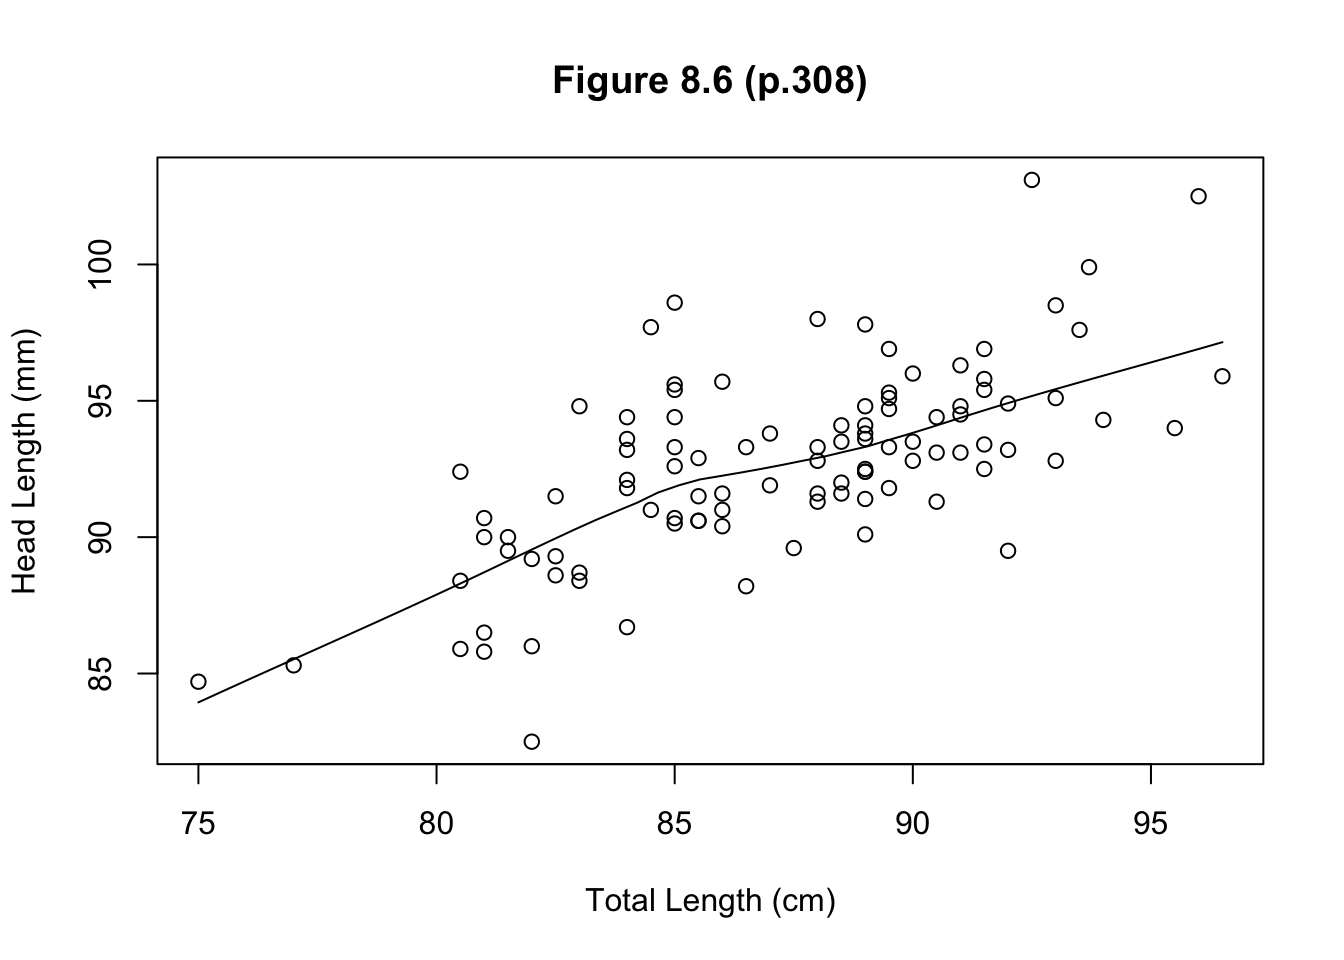
\includegraphics{Problem-Set-1-Answer-Key_files/figure-latex/unnamed-chunk-13-1.pdf}

\hypertarget{box-plot-check-for-outliers}{%
\subsection{Box Plot: Check for Outliers}\label{box-plot-check-for-outliers}}

Make box plots for x (total\_l) and y (head\_l), respectively.

\begin{Shaded}
\begin{Highlighting}[]
\KeywordTok{boxplot}\NormalTok{(x, }\DataTypeTok{main =} \StringTok{"Box Plot of Total Length (cm)"}\NormalTok{)}
\end{Highlighting}
\end{Shaded}

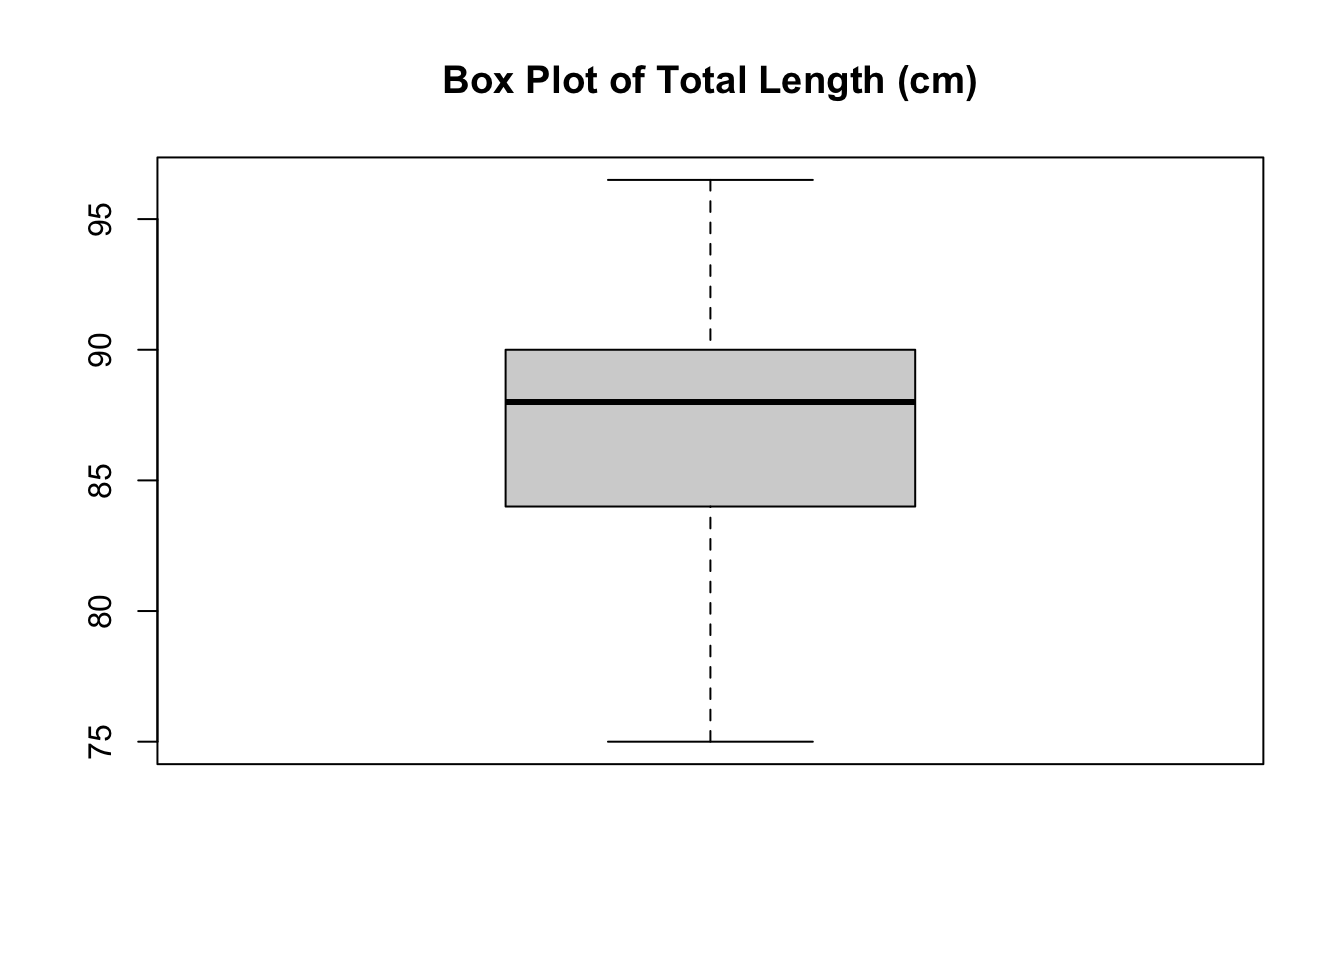
\includegraphics{Problem-Set-1-Answer-Key_files/figure-latex/unnamed-chunk-14-1.pdf}

\begin{Shaded}
\begin{Highlighting}[]
\KeywordTok{boxplot}\NormalTok{(y, }\DataTypeTok{main =} \StringTok{"Box Plot of Head Length (mm)"}\NormalTok{)}
\end{Highlighting}
\end{Shaded}

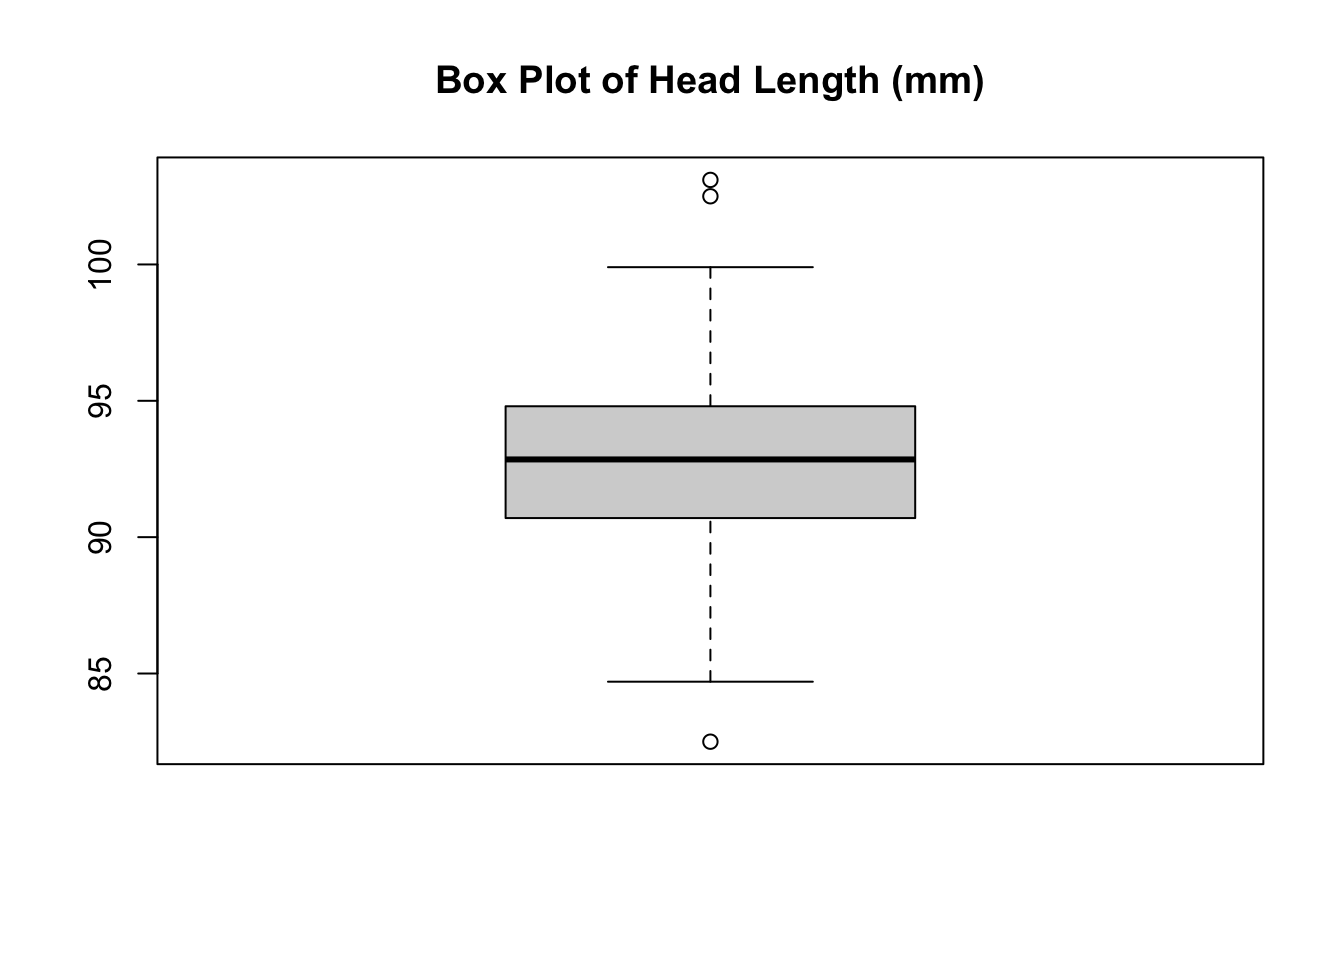
\includegraphics{Problem-Set-1-Answer-Key_files/figure-latex/unnamed-chunk-14-2.pdf}

\hypertarget{density-plot-check-for-normality}{%
\subsection{Density Plot: Check for Normality}\label{density-plot-check-for-normality}}

Make density plots for x (total\_l) and y (head\_l), respectively.

\begin{Shaded}
\begin{Highlighting}[]
\KeywordTok{plot}\NormalTok{(}\KeywordTok{density}\NormalTok{(x), }\DataTypeTok{main =} \StringTok{"Density Plot of Total Length (cm)"}\NormalTok{)}
\end{Highlighting}
\end{Shaded}

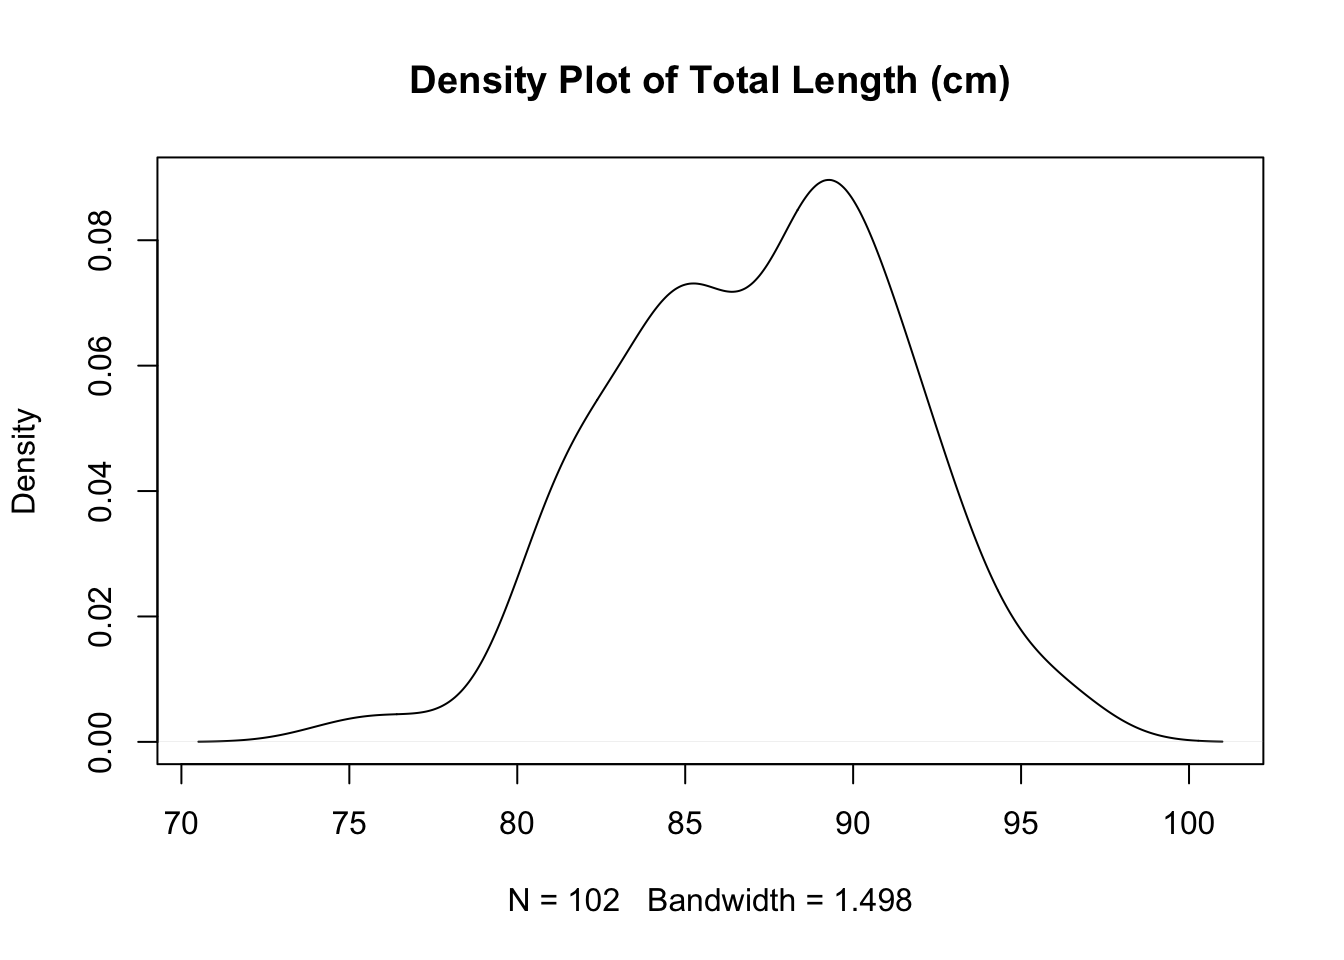
\includegraphics{Problem-Set-1-Answer-Key_files/figure-latex/unnamed-chunk-15-1.pdf}

\begin{Shaded}
\begin{Highlighting}[]
\KeywordTok{plot}\NormalTok{(}\KeywordTok{density}\NormalTok{(y), }\DataTypeTok{main =} \StringTok{"Density Plot of Head Length (mm)"}\NormalTok{)}
\end{Highlighting}
\end{Shaded}

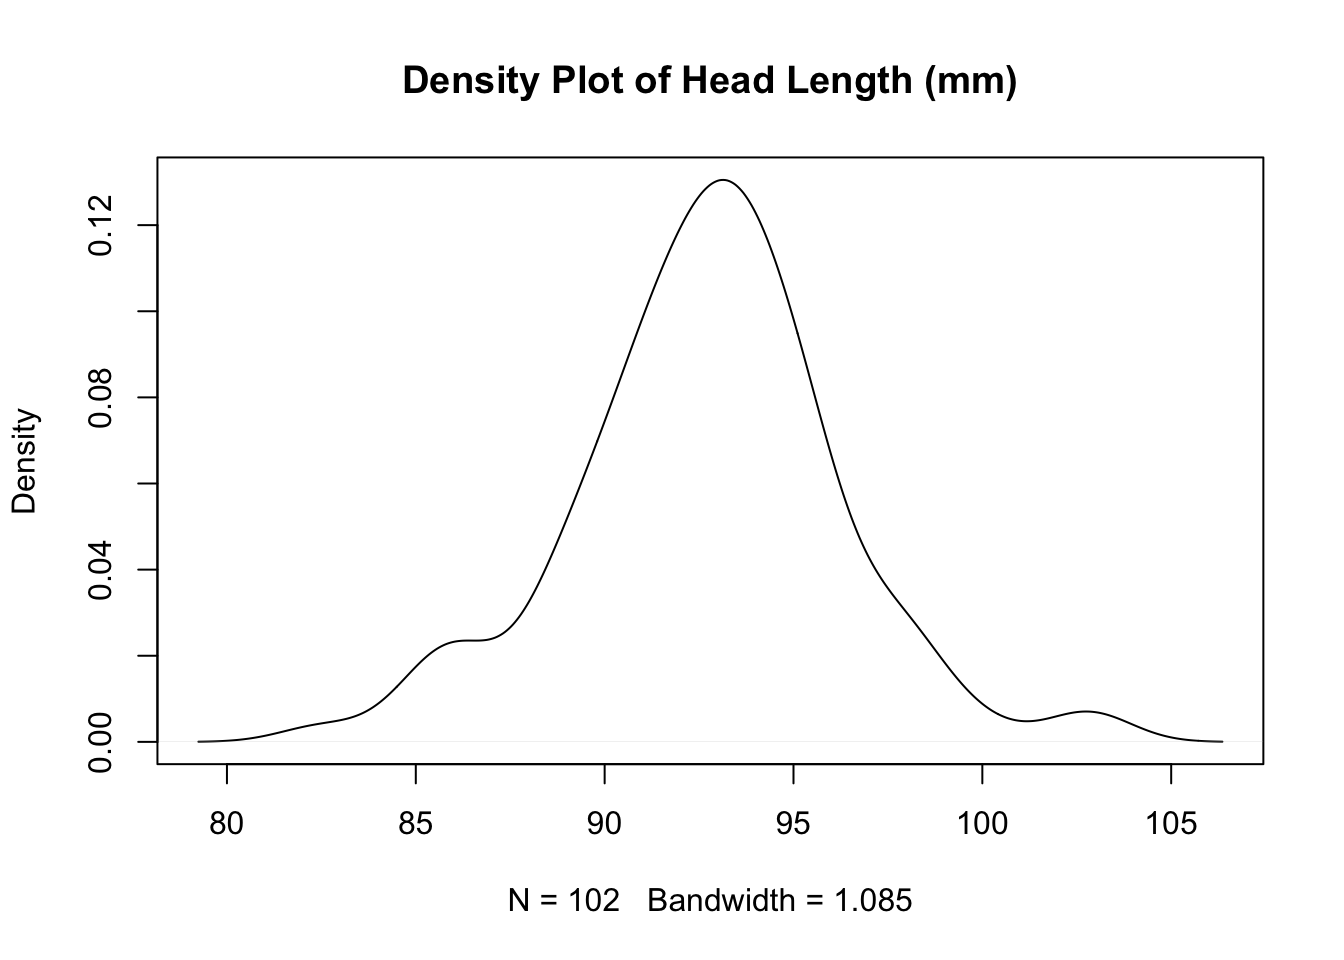
\includegraphics{Problem-Set-1-Answer-Key_files/figure-latex/unnamed-chunk-15-2.pdf}

\hypertarget{linear-regression}{%
\section{Linear Regression}\label{linear-regression}}

\hypertarget{model}{%
\subsection{Model}\label{model}}

Fit the least squares regression

\begin{align}
head_l = \beta_0 + \beta_1 total_l + e.
\end{align}

\begin{Shaded}
\begin{Highlighting}[]
\CommentTok{# y ~ x}
\NormalTok{fit <-}\StringTok{ }\KeywordTok{lm}\NormalTok{(head_l }\OperatorTok{~}\StringTok{ }\NormalTok{total_l, }\DataTypeTok{data =}\NormalTok{ possum_new)}

\KeywordTok{summary}\NormalTok{(fit)}
\end{Highlighting}
\end{Shaded}

\begin{verbatim}
## 
## Call:
## lm(formula = head_l ~ total_l, data = possum_new)
## 
## Residuals:
##    Min     1Q Median     3Q    Max 
## -7.226 -1.593 -0.326  1.303  7.424 
## 
## Coefficients:
##             Estimate Std. Error t value Pr(>|t|)    
## (Intercept) 43.25900    5.41959   7.982 2.49e-12 ***
## total_l      0.56667    0.06206   9.131 7.95e-15 ***
## ---
## Signif. codes:  0 '***' 0.001 '**' 0.01 '*' 0.05 '.' 0.1 ' ' 1
## 
## Residual standard error: 2.618 on 100 degrees of freedom
## Multiple R-squared:  0.4547, Adjusted R-squared:  0.4492 
## F-statistic: 83.37 on 1 and 100 DF,  p-value: 7.946e-15
\end{verbatim}

We have

\begin{align}
\hat{\beta}_0 & = 43.25900 \\
\hat{\beta}_1 & = 0.56667.
\end{align}

\hypertarget{residual-analysis}{%
\subsection{Residual Analysis}\label{residual-analysis}}

Make a scatterplot and a residual plot for regression. Discuss whether fitting a linear model would be appropriate.

\begin{Shaded}
\begin{Highlighting}[]
\CommentTok{# scatterplot}
\KeywordTok{scatter.smooth}\NormalTok{(}\DataTypeTok{x =}\NormalTok{ x, }\DataTypeTok{y =}\NormalTok{ y, }
               \DataTypeTok{xlab =} \StringTok{"Total Length (cm)"}\NormalTok{, }
               \DataTypeTok{ylab =} \StringTok{"Head Length (mm)"}\NormalTok{, }
               \DataTypeTok{main =} \StringTok{"Scatterplot - Figure 8.6 (p.308)"}\NormalTok{) }
\end{Highlighting}
\end{Shaded}

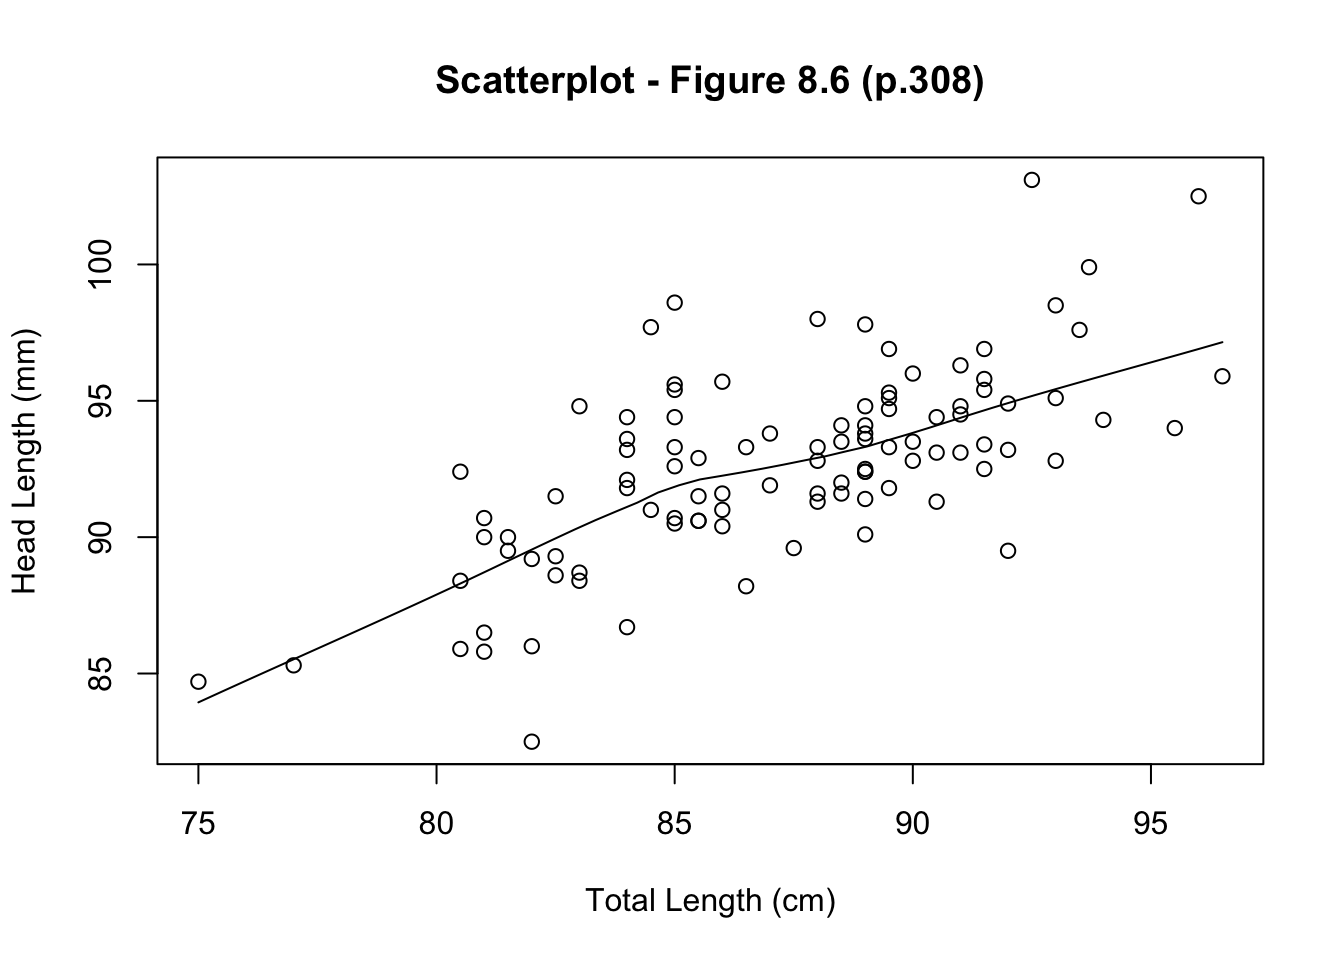
\includegraphics{Problem-Set-1-Answer-Key_files/figure-latex/unnamed-chunk-17-1.pdf}

\begin{Shaded}
\begin{Highlighting}[]
\CommentTok{# residual plot}
\KeywordTok{plot}\NormalTok{(}\DataTypeTok{x =}\NormalTok{ possum_new}\OperatorTok{$}\NormalTok{total_l, }\DataTypeTok{y =}\NormalTok{ fit}\OperatorTok{$}\NormalTok{residuals,}
     \DataTypeTok{xlab =} \StringTok{"Total Length (cm)"}\NormalTok{,}
     \DataTypeTok{ylab =} \StringTok{"Residuals"}\NormalTok{,}
     \DataTypeTok{main =} \StringTok{"Residual Plot - Figure 8.7 (p.309)"}\NormalTok{)}
\KeywordTok{abline}\NormalTok{(}\DataTypeTok{h=}\DecValTok{0}\NormalTok{)}
\end{Highlighting}
\end{Shaded}

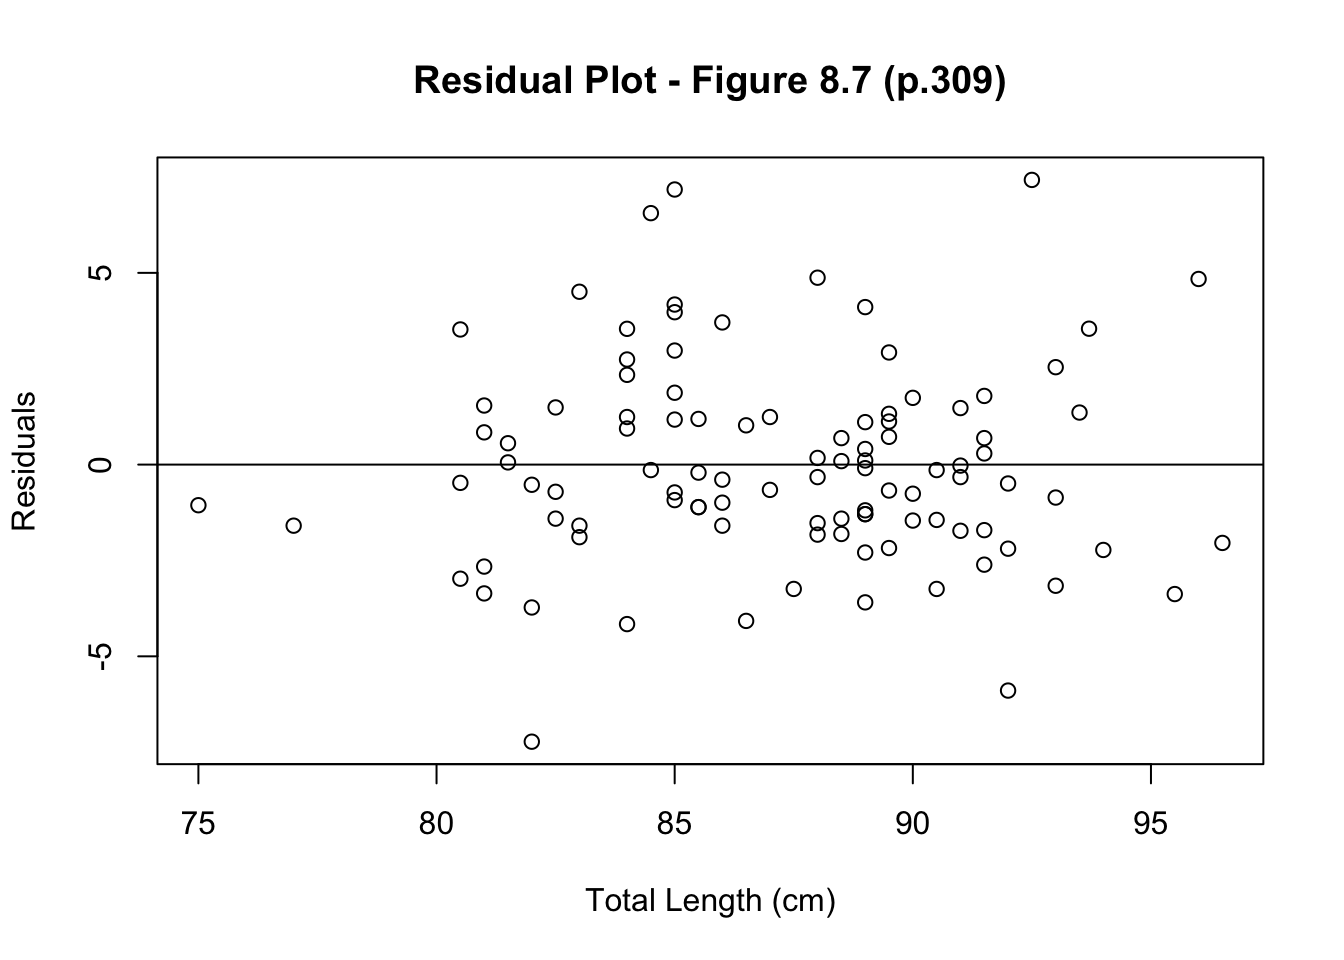
\includegraphics{Problem-Set-1-Answer-Key_files/figure-latex/unnamed-chunk-17-2.pdf}

\begin{Shaded}
\begin{Highlighting}[]
\CommentTok{# density plot}
\KeywordTok{plot}\NormalTok{(}\KeywordTok{density}\NormalTok{(fit}\OperatorTok{$}\NormalTok{residuals), }\DataTypeTok{main =} \StringTok{"Density Plot of Residuals"}\NormalTok{)}
\end{Highlighting}
\end{Shaded}

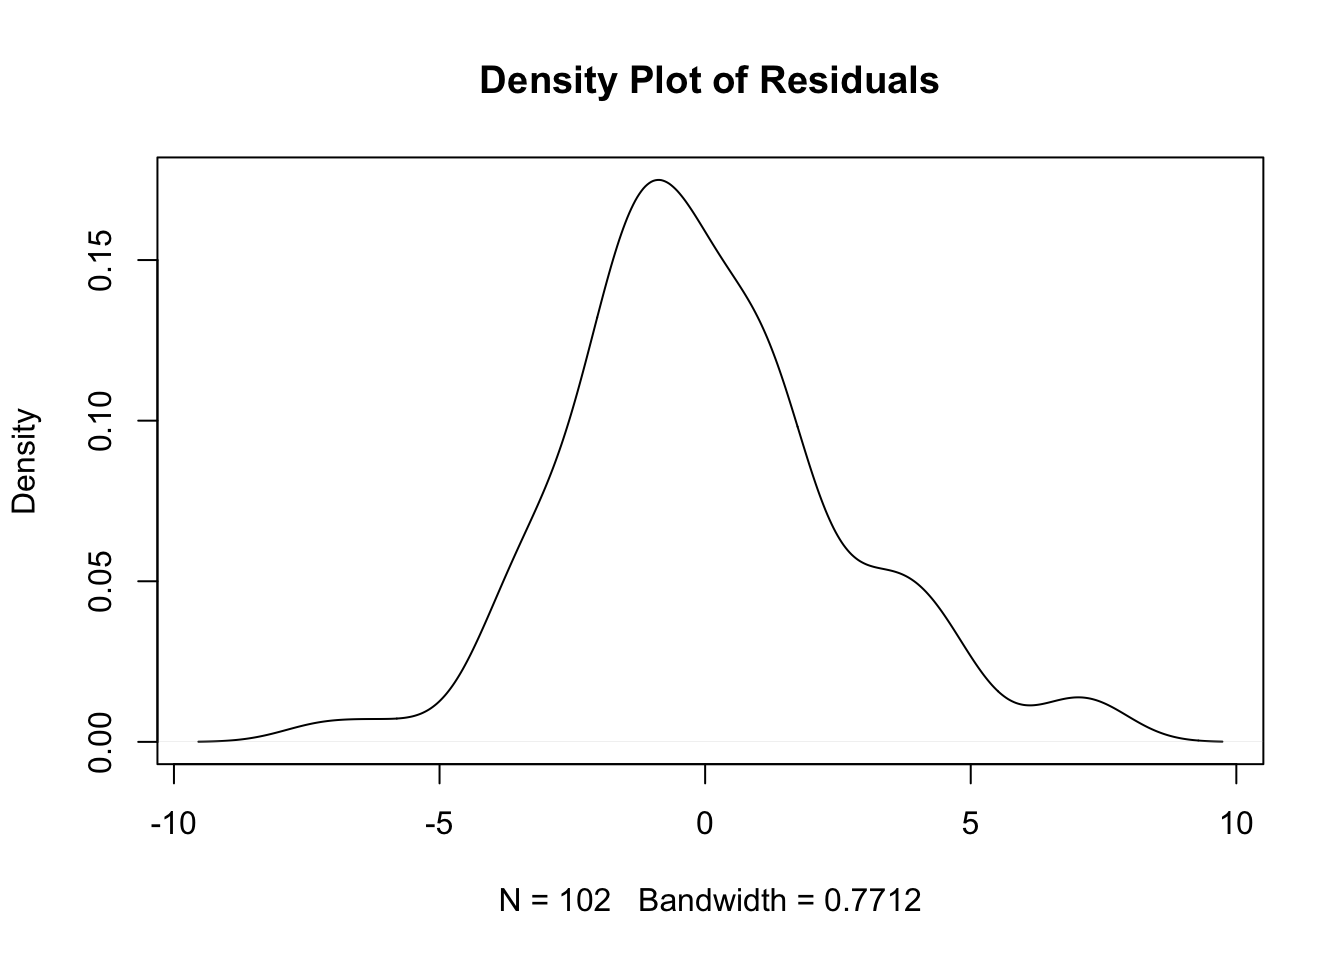
\includegraphics{Problem-Set-1-Answer-Key_files/figure-latex/unnamed-chunk-17-3.pdf}

Check the following conditions:

\begin{itemize}
\item
  Linearity: linear trend, i.e., no patterns in residual plot. (valid)
\item
  Normal residuals: no extremely large or small residuals. (valid)
\item
  Constant variability: points around line dispersed in similar way. (valid)
\item
  Independent observations: occurrence of one observation provides no information about occurence of the other. (valid)
\end{itemize}

Thus, fitting a linear model would be appropriate for this case.

  \bibliography{book.bib,packages.bib}

\end{document}
